\begin{titlepage}

    \begin{center}

        
\includegraphics[width=0.6\textwidth]{figures/苏州大学.png}
        \vspace{5ex}
        \fontsize{32pt}{1.2em}\selectfont

        \textbf{本\ 科\ 毕\ 业\ 设\ 计\ (\ 论\ 文\ )}
        \vspace{1.2em}
        \vspace{8ex}
        \zihao{4}

        \begin{tabular}{lcll}
            学院(部)  & \multicolumn{3}{c}{\textsf{魔法学院}}
            \\ \cline{2-4}
            题目        & \multicolumn{3}{>{\centering\arraybackslash}p{9cm}}{\textsf{从圣光之子到冰封王座:论阿尔萨斯·米奈希尔的堕落与巫妖王身份的跨维度构建}}
            \\ \cline{2-4}
            年级        & \multicolumn{1}{l}{\textsf{2021}}                 & 专业  & \textsf{魔法学} 
            \\ \cline{2-2} \cline{4-4}
            班级        & \multicolumn{1}{l}{\textsf{21魔法}}               & 学号  & \textsf{2000000000}   
            \\ \cline{2-2} \cline{4-4}
            姓名        & \multicolumn{3}{c}{\textsf{吉安娜·普罗德摩尔}}                            
            \\ \cline{2-4}
            指导老师    & \multicolumn{1}{l}{\textsf{安东尼达斯}}           & 职称  & \textsf{大法师}         
            \\ \cline{2-2} \cline{4-4}
            论文提交日期& \multicolumn{3}{c}{\textsf{2025年5月1日}}                                     
            \\ \cline{2-4}
        \end{tabular}

    \end{center}

\end{titlepage}


% 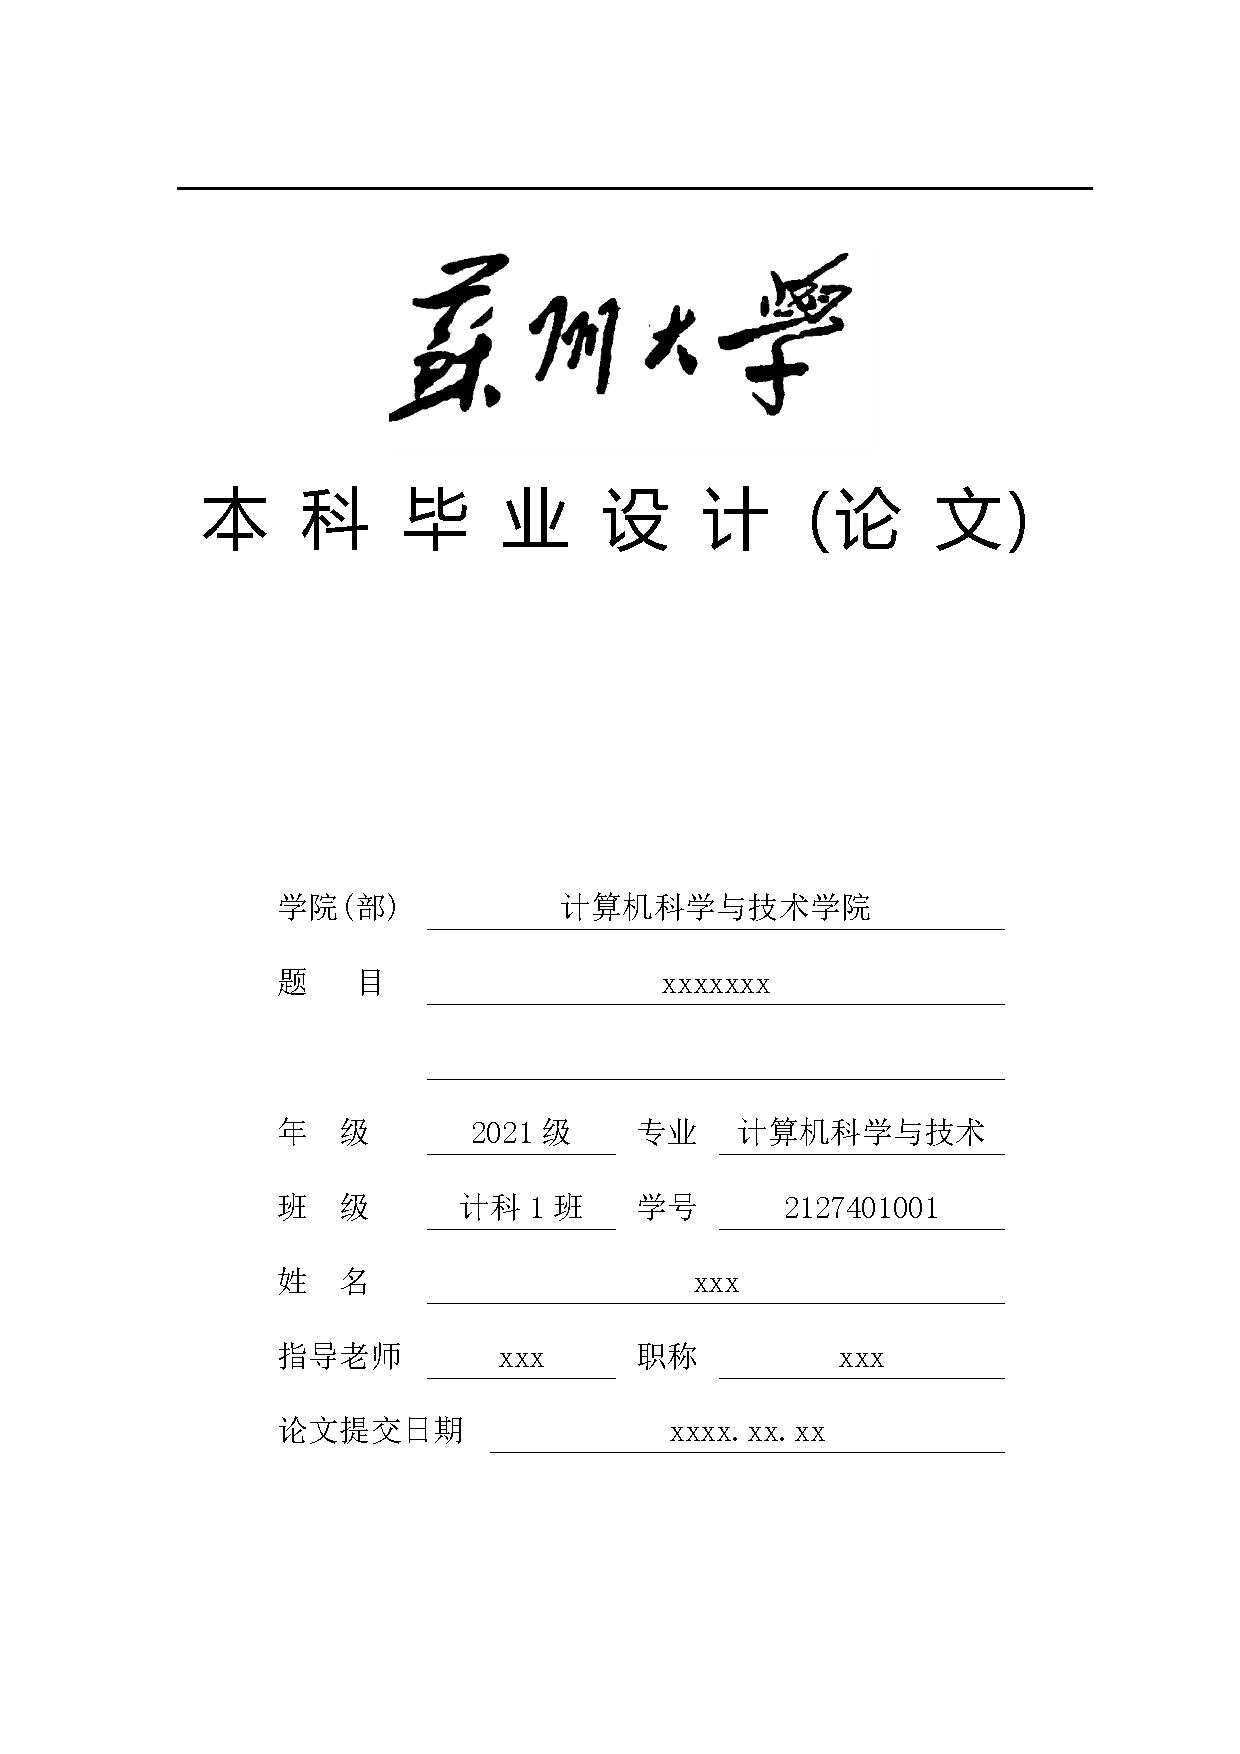
\includepdf{figure/封面.pdg}
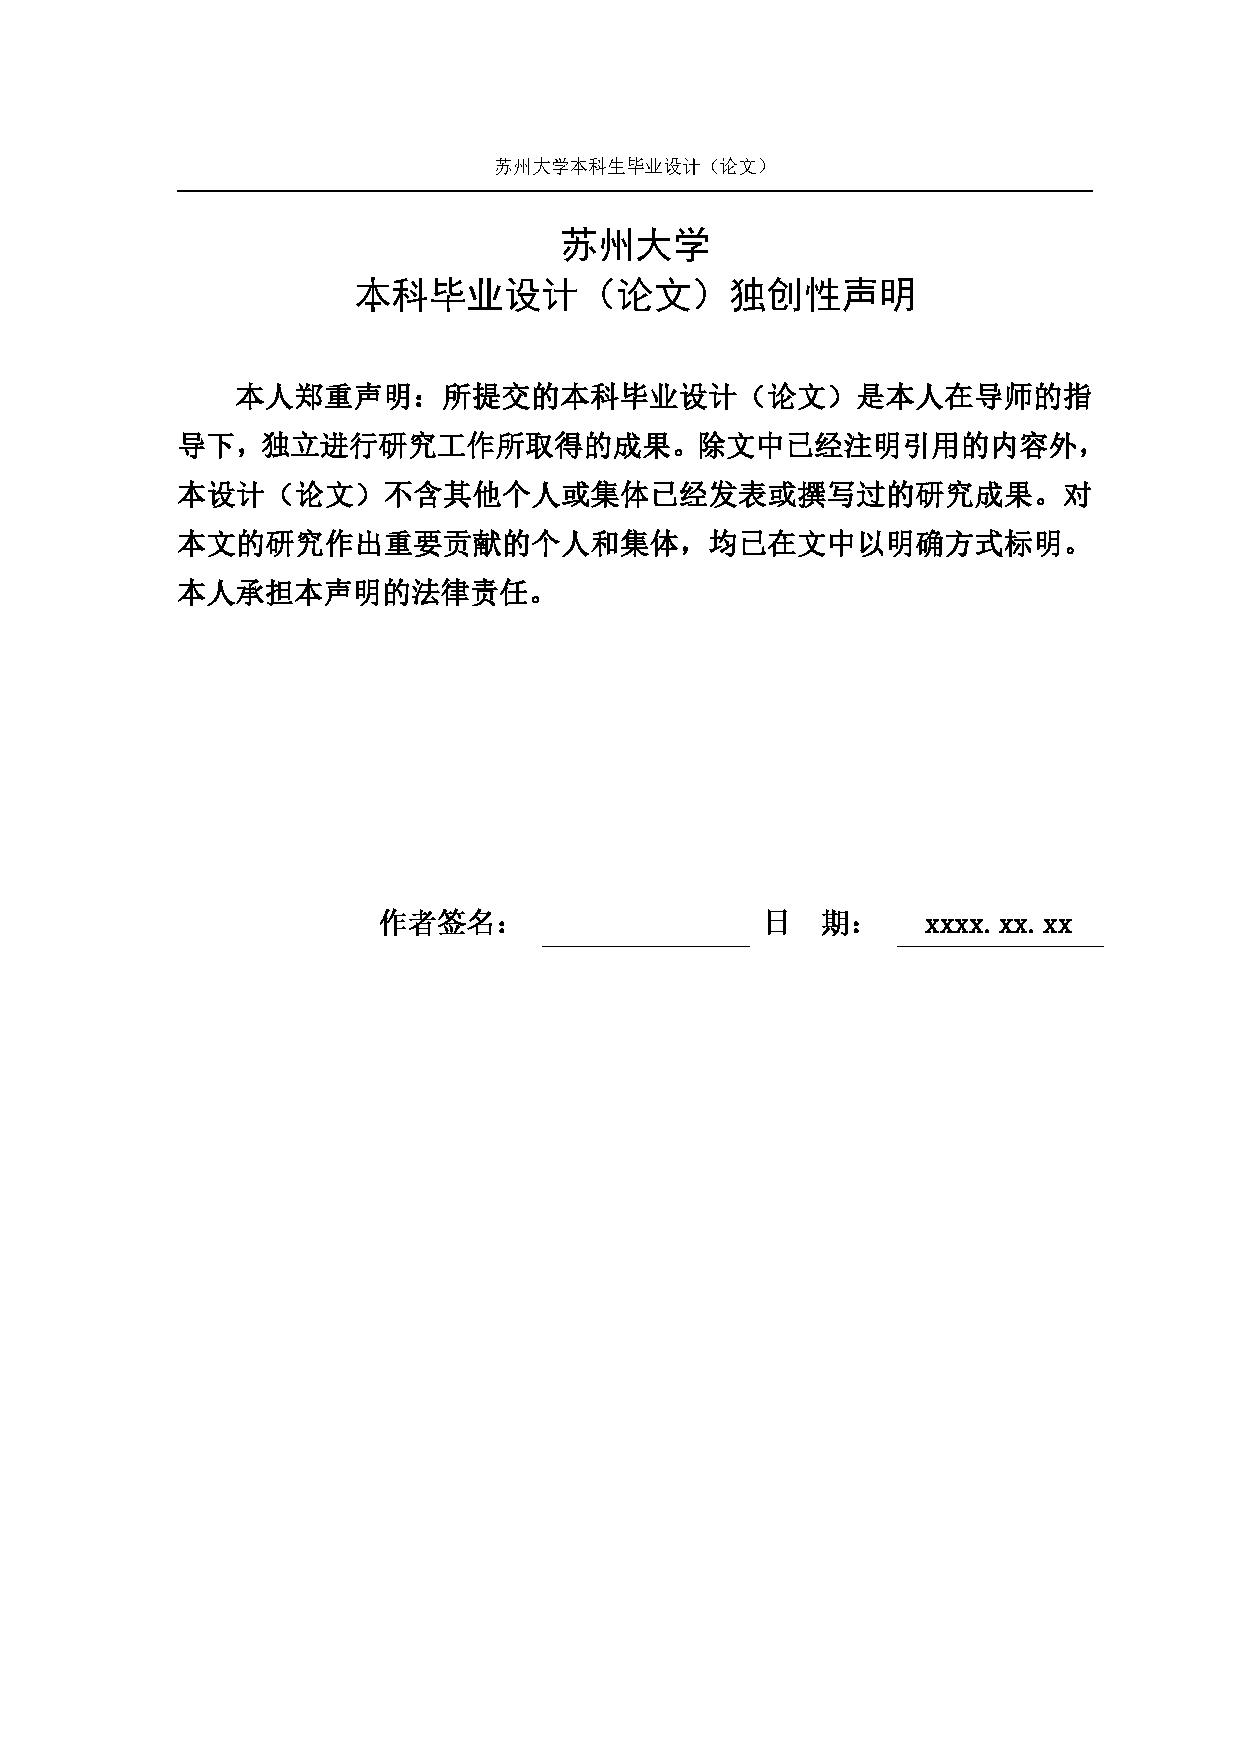
\includepdf{figures/独创性说明.pdf}
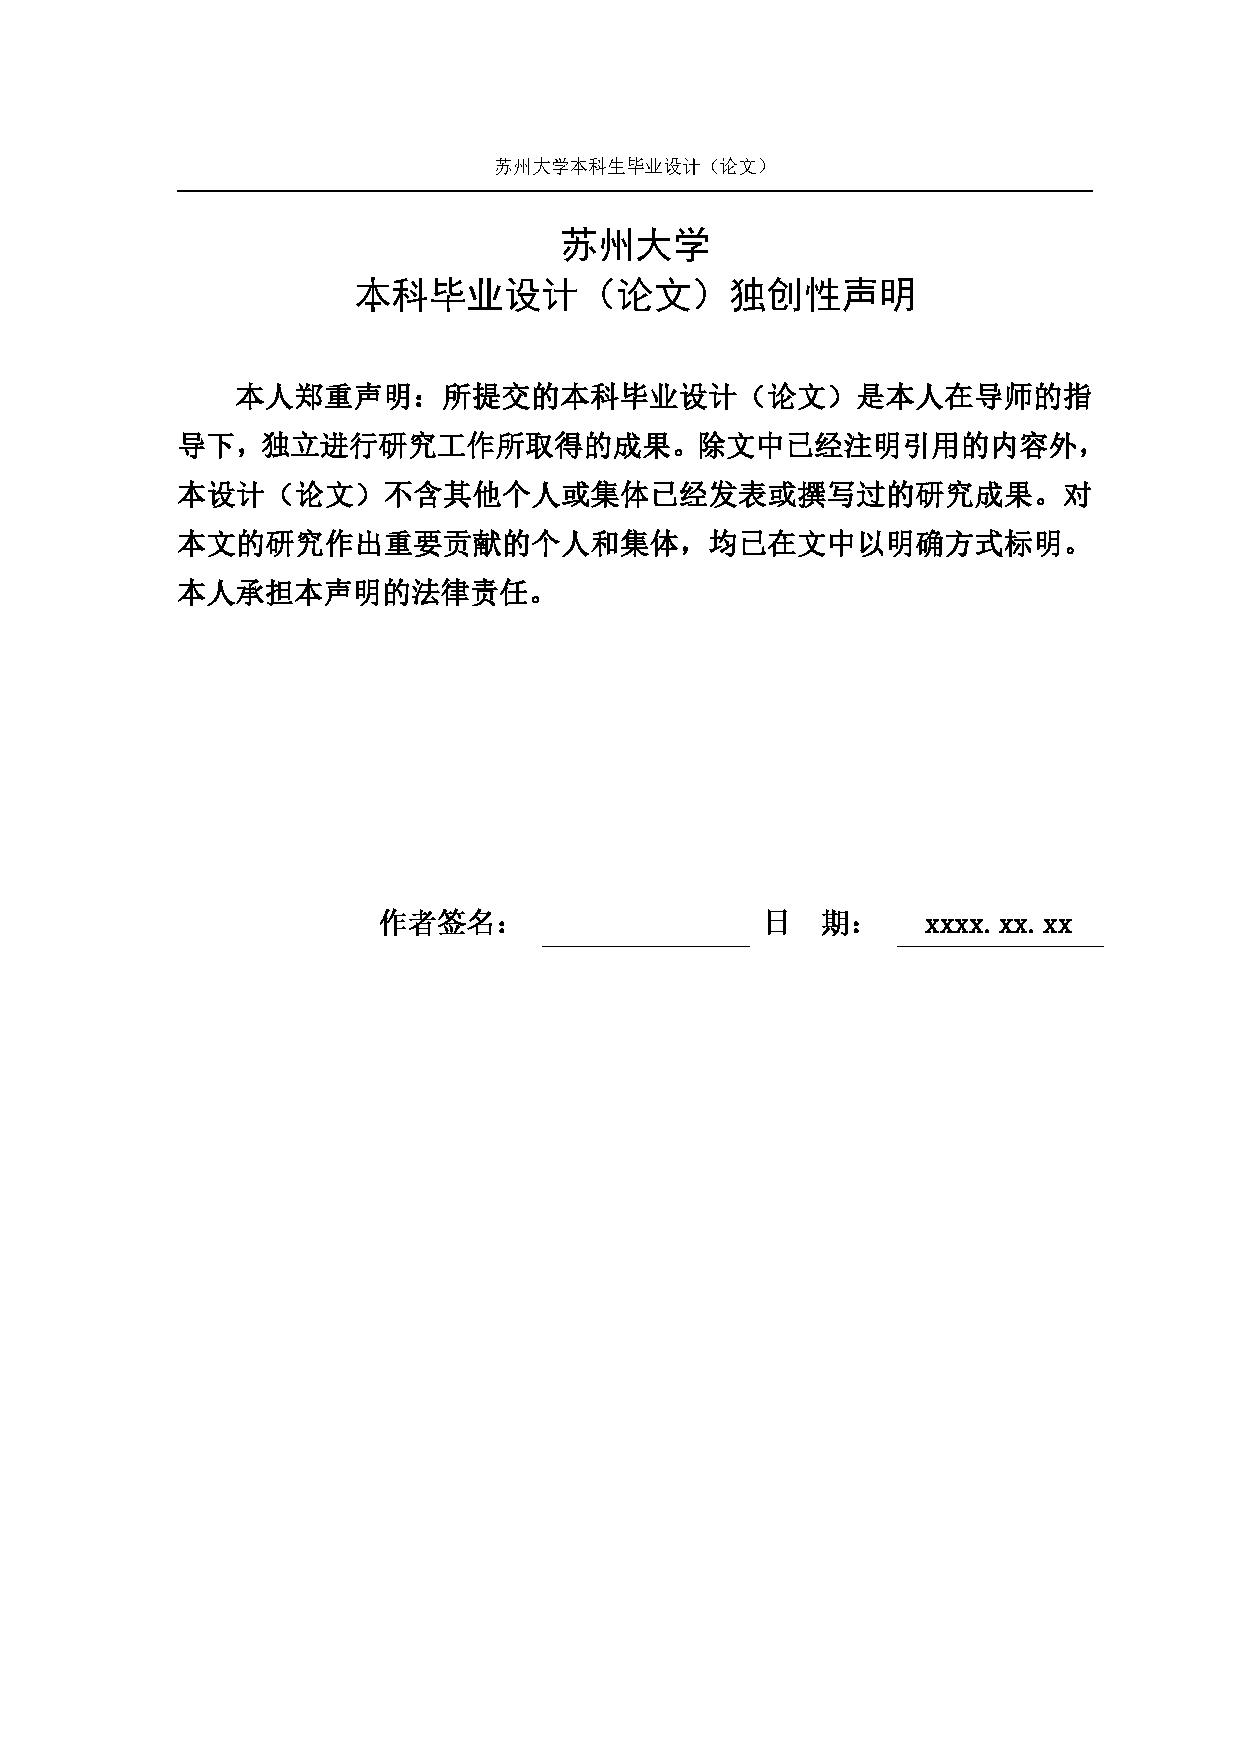
\includepdf{figures/独创性说明.pdf}

